\title{SE2 CheatSheet}
\author{dthoma}
\date{August 2017}

\documentclass[a4paper, fontsize=6pt]{scrartcl}
\usepackage{multicol}
\usepackage{calc}
\usepackage{ifthen}
\usepackage[landscape]{geometry}
\usepackage{hyperref}
\usepackage{graphicx}
\usepackage{mathtools}
\usepackage{gensymb}
\usepackage{minted}
\usemintedstyle{bw}
\usepackage{ragged2e} 
\usepackage[T1]{fontenc}
\usepackage[utf8]{inputenc}
\usepackage{amsbsy}
\usepackage{amsfonts}
\usepackage{varwidth,pst-tree,pst-eps}
\usepackage{comment}
\usepackage{xcolor}

\usepackage{fontspec}

\setromanfont[
Path=fonts/Roboto/,
BoldFont=Roboto-Bold.ttf,
ItalicFont=Roboto-Italic.ttf,
BoldItalicFont=Roboto-BoldItalic.ttf
]{Roboto-Regular.ttf}
\setmonofont[
Path=fonts/Hack/,
BoldFont=Hack-Bold.ttf,
ItalicFont=Hack-Italic.ttf,
BoldItalicFont=Hack-BoldItalic.ttf
]{Hack-Regular.ttf}

\AtBeginEnvironment{minted}{%
  \renewcommand{\fcolorbox}[4][]{#4}}

%German-specific commands
%--------------------------------------
\usepackage[german]{babel}
%--------------------------------------

\graphicspath{ {images/} }


% This sets page margins to .5 inch if using letter paper, and to 1cm
% if using A4 paper. (This probably isn't strictly necessary.)
% If using another size paper, use default 1cm margins.
\geometry{top=0.5cm,left=0.5cm,right=0.5cm,bottom=0.5cm}

% Turn off header and footer
\pagestyle{empty}
 

% Redefine section commands to use less space
\makeatletter
\renewcommand{\section}{\@startsection{section}{1}{0mm}%
    {-1ex plus -.5ex minus -.2ex}%
    {0.5ex plus .2ex}%x
    {\normalfont\large\bfseries}}
    
\renewcommand{\subsection}{\@startsection{subsection}{2}{0mm}%
    {-1explus -.5ex minus -.2ex}%
    {0.5ex plus .2ex}%
    {\normalfont\normalsize\bfseries}}
    
\renewcommand{\subsubsection}{\@startsection{subsubsection}{3}{0mm}%
    {-1ex plus -.5ex minus -.2ex}%
    {1ex plus .2ex}%
    {\normalfont\small\bfseries}}
    
\makeatother

% Define BibTeX command
\def\BibTeX{{\rm B\kern-.05em{\sc i\kern-.025em b}\kern-.08em
    T\kern-.1667em\lower.7ex\hbox{E}\kern-.125emX}}

% Don't print section numbers
%\setcounter{secnumdepth}{0}


\setlength{\parindent}{0pt}
\setlength{\parskip}{0pt plus 0.5ex}


% -----------------------------------------------------------------------

\begin{document}

\footnotesize
\begin{multicols*}{5}


% multicol parameters
% These lengths are set only within the two main columns
%\setlength{\columnseprule}{0.25pt}
\setlength{\premulticols}{1pt}
\setlength{\postmulticols}{1pt}
\setlength{\multicolsep}{1pt}
\setlength{\columnsep}{2pt}

Partnerarbeit von dthoma und lroellin

\section{HTML5}
HTML ist a document markup language: markup = semantic annotation of information

Declarative: Defines a meaning => semantic annotation

May be translated into different outputs

\textbf{Void elements}: area, base, br, col, command, embed, hr, img, input, keygen, link, meta, param, source, track, wbr

\textbf{Optional closing:} html, head, body, p, dt, dd, li, option, thead, th, tbody, tr, td, tfoot, colgroup

\textbf{Attributes:} \mintinline{html}{data-} allow custom attributes

\subsection{Document Structure}
\begin{minted}{html}
<!DOCTYPE html>
<html lang="en">
  <!-- comment -->
  <head>
    <title></title>
    <meta charset="utf-8">
  </head>
  <body>
    <header><time datetime=></time></header>
    <nav></nav>
    <main><figure><img/><figcaption></figcaption></main>
    <footer><video src= poster= controls></video></footer>
  </body>
  <script src=""></script>
</html>
\end{minted}

\textbf{Document Type}: \mintinline{html}{<!DOCTYPE html>} Standard Mode (HTML5), alles andere => quirks mode (compatibility mode)

\subsection{Content Structure}
\subsubsection{Content Areas}
\textbf{section:} Semantic section (e.g. chapter, topic)

\textbf{aside:} Side content, (additional information)

\textbf{article:} Complete article, post => containing header, footer, text, author, 

\textbf{header, footer:} Header or footer of document, section, article, ...

\textbf{main:} Main section of the document (Use only once!)

\subsubsection{Headings 1-6}

\subsubsection{Text}
\textbf{p:} (Paragraph) Text paragraph, may contain line breaks <br />

\textbf{small:} (Small annotations) Small prints, legal notice

\textbf{time, address, abbr, blockquote, cite, pre, code:} Time, address (contact only), abbrevation, blockquote, cite, plain text and code markup

\textbf{strong, em:} Important content / emphasized content

\textbf{hr:} Paragraph-level thematic break

\subsubsection{Other Tags}
\textbf{i:} (names, terms) Other content without additional meaning

\textbf{b:} Stylistically different content

\textbf{div:} General tag to group other flow content.

\textbf{span:} General tag to group phrasing content, used for styling.

\subsubsection{Navigation}
nav: Main navigation section
not for aside menus, language menus or footer menus

\subsubsection{Link (anchor)}
Must not contain interactive elements (input, button, a)

Wichtige Attribute: \mintinline{html}{target}, \mintinline{html}{download}, \mintinline{html}{type} (MIME)

\subsection{Lists}
ul, ol, dl

\subsubsection{ol}
\textbf{start:} Numbering start value

\textbf{reversed:} Reverse ordering

\textbf{value:} List point value (cont. numbering)

\subsubsection{dl (definition list)}
\textbf{dt:} term

\textbf{dd:} definition

\begin{minted}{html}
<dl>
<dt>Airplane</dt>
<dd>Vehicle to fly</dd>
<dd>Also called <i>Aircraft</i></dd>
</dl>
\end{minted}

\subsection{Tables}
\begin{minted}{html}
<table>
  <tr>
    <th>true</th>
    <td>true</td>
  </tr>
</table>
\end{minted}
\begin{tabular}{|p{0.26\linewidth}|p{0.6\linewidth}|}
 \hline
 thead, tbody, tfoot & Table header, body and footer (optional) \\ 
 tr & Table row (may be empty) \\ 
 th/td & Table header cell (head, body) / data cell (body) \\ 
 \hline
\end{tabular}

\subsection{Images}
\begin{minted}{html}
<img alt="..." longdesc="link-to-desc.tld" 
  src="Titelbild_Abend-1200.jpg"
  srcset="Titelbild_Abend-320.jpg 320w, 
          Titelbild_Abend-640.jpg 640w,
          Titelbild_Abend-1200.jpg 1200w"
  sizes="100vw">
\end{minted}
For normal cases: use img instead

\textbf{img:} Browser may handle images smart.

\textbf{picture:} Browser needs to follow the rules (no smart enhancements).

\subsection{Forms}
\begin{minted}{html}
<form action="./sendMessage" method="post">
 <label for="name">Name</label>
  <input type="text" name="name" id="name">
 <select name="m" id="m" size="1">
  <option value="feedback" selected>Feeb.</option>
  <option value="question">Question</option>
 </select>
 <textarea name="textarea"
  rows="10" cols="50">text</textarea>
 <button type="submit">Send request</button>
\end{minted}


\subsection{Content Model}

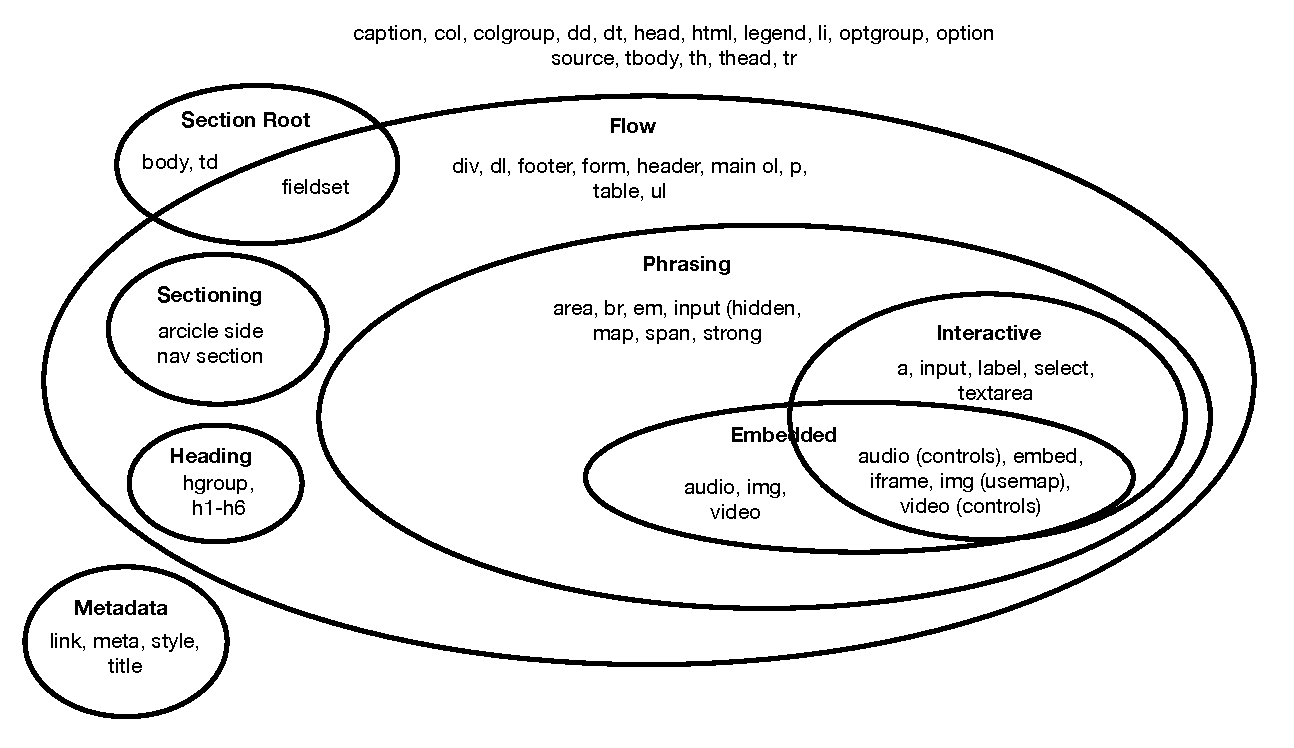
\includegraphics[scale = 0.27]{contentmodel.pdf}

\section{CSS - Cascading Style Sheets}

CSS wurde entworfen um ein einheitliches und wiederverwendbares Styling Tool zu Verfügung zu stellen. Mit HTML5 wurden alle Style Tags als deprecated eingestuft und dürfen nicht mehr verwendet werden.

\begin{minted}{css}
<style>span{ background: red; }</style>
<link rel="stylesheet" href="f.css" media="screen">
\end{minted}

\subsection{Selektoren}

Bei CSS beginnt der Index bei 1. 2n selektiert alle Indizes $i \equiv 0 \mod 2$.

\begin{tabular}{ |c|c| } 
 \hline
 Universal & \mintinline{css}{* { }} \\ 
 Attribute & \mintinline{css}{a[href=".pdf"] { }} \\ 
 Pseudo-Elemente & \mintinline{css}{a::before { }} \\ 
 Attribute & \mintinline{css}{tr:nth-child(2n){ }} \\ 
 Kindselektor (direkte Kinder) & \mintinline{css}{e > f} \\ 
 Nachfahrenselektor & \mintinline{css}{e f} \\ 
 Nachbarselektor (nächster) & \mintinline{css}{e + f} \\ 
 Geschwisterselektor & \mintinline{css}{e ~ f} \\ 
 \hline
\end{tabular}

\subsection{Attributsprüfungen}

\begin{tabular}{ |c|c| } 
 \hline
 \mintinline{css}{a=v} & Attribut a gleich Wert v (komplett) \\ 
 \mintinline{css}{a~=v} & a beinhaltet v (alleinstehend) \\ 
 \mintinline{css}{a|=v} & a startet mit v (alleinstehend) \\ 
 \mintinline{css}{a^=v} & a startet mit v \\
 \mintinline{css}{a^=v} & a startet mit v \\
 \mintinline{css}{a$=v} & a endet mit v \\
 \mintinline{css}{a*=v} & a beinhaltet v \\
 \hline
\end{tabular}

\subsubsection{Pseudoelemente}
\begin{tabular}{|p{0.25\linewidth}|p{0.6\linewidth}|} 
 \hline
 \mintinline{css}{::first-line} & Selektiert die erste Textzeile \\ 
 \mintinline{css}{::first-letter} & Selektiert den ersten Buchstaben \\ 
 \mintinline{css}{::before ::after} & erzeugen ein neues Element, \mintinline{css}{content:} und \mintinline{css}{display: inline-block}\\ 
 \mintinline{css}{::selection} & Farbe der Selektion anpassen \\ 
 \hline
\end{tabular}

\subsubsection{Pseudoklassen}
\begin{tabular}{|p{0.6\linewidth}|p{0.2\linewidth}|}
 \hline
 \mintinline{css}{:first-child :nth-child() :empty} & strukturell \\ 
 \mintinline{css}{:hover :active :focus :visited} & dynamisch \\ 
 \mintinline{css}{:lang() :not() :matches()} & divers \\ 
 \hline
\end{tabular}

\subsection{Box Model}

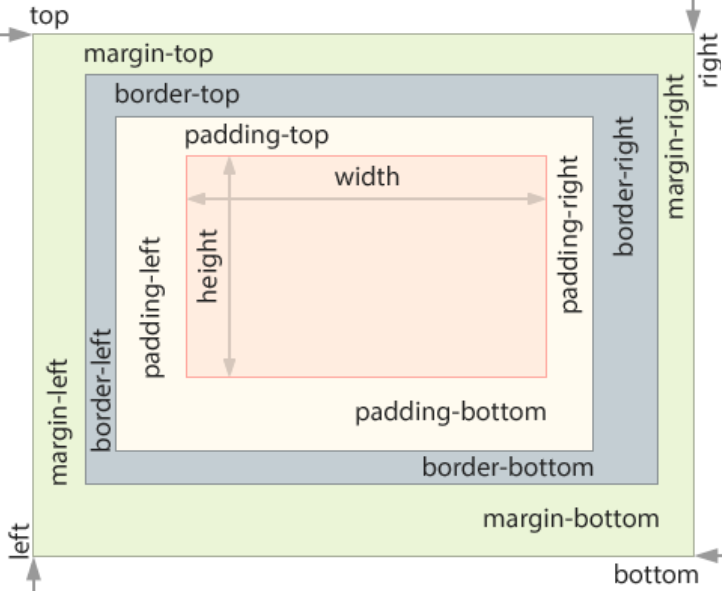
\includegraphics[scale = 0.16]{box-model-cropped.png}

Mit \mintinline{css}{box-sizing: border-box;} und einer Breite von 100px entspricht die Breite des Elements 100px mit Content, Border und Padding.

Mit \mintinline{css}{box-sizing: content-box;} und einer Breite von 100px entspricht die Breite des Elements 100px mit Content und ohne Border und Padding.

\mintinline{css}{margin: 1px 2px 3px 4px;} ( top | right | bottom | left – Uhrzeigersinn)

\subsection{Position}

Mit ''Position'' kann ein Element aus dem Fluss genommen werden. Absolute und Fixed reservieren keinen Platz. Relative jedoch schon.

\subsection{Kaskade}

Zähler \textbf{A} erhöht sich durch: ID-Selektor (\#). Zähler \textbf{B} durch Attribut- oder Klassenselektor, bzw. Pseudoklassen. Zähler \textbf{C} durch Typselektor oder Pseudoelemente. 

Selektoren innerhalb von \mintinline{css}{:not()} werden wie alle anderen gezählt, \mintinline{css}{:not()} selber jedoch nicht. Universalselektor \mintinline{css}{*} wird komplett ignoriert.

Daneben gibt es noch ein spezifischeres Argument. Hat ein Element ein \mintinline{html}{style=} Attribut, so gelten diese Regeln spezifischer als alle anderen (Zähler vor A)

\subsection{Einheiten}

\textbf{px:} Ist die Basis-Einheit vom Browser.

\textbf{em:} Relativ zur Parent-Schriftgrösse.

\textbf{rem:} Relativ zur Root-Element (html).

\textbf{vw/vh:} \%-Grösse vom Viewport.

\subsection{Font}
\begin{tabular}{|p{0.3\linewidth}|p{0.5\linewidth}|}
 \hline
 \mintinline{css}{font-family:} & Die erste vom Browser unterstützte Schriftart. \\ 
 \mintinline{css}{font-style:} & italic, oblique \\ 
 \mintinline{css}{font-variant:} & small-caps \\ 
 \mintinline{css}{font-size:} & Grösse \\ 
 \mintinline{css}{font-weight:} & 100-900, bold, ... \\ 
 \mintinline{css}{line-height:} & Zeilenhöhe \\ 
 \mintinline{css}{text-decoration:} & underline, overline, line-through \\ 
 \hline
\end{tabular}

\section{JavaScript}

ECMAScript ist der offizielle Name für JavaScript. \\

Standard JS-Dateibeginn, für alles was erst nach dem DOM laufen soll:

\begin{minted}{js}
window.onload = () => {/* code */}
// oder (jQuery)
$(function() {/* code */});
\end{minted}

Will man \mintinline{js}{$} festlegen, es könnte ja auch etwas anderes als jQuery sein, baut man folgendes um diesen Scope:

\begin{minted}{js}
(function ($) {/* code */})(jquery)
\end{minted}

\mintinline{js}{eval()} ist evil!

\subsection{Operatoren}
Bei Gleichwertigkeit: von links nach rechts!

\subsection{Boolean}

'falsy' Werte: false, 0, ''''. null, undefined, NaN \\
'truthy' Werte: alles andere ('0', 'false', \{\}, [])

Strings werden lexikographisch verglichen. A kommt vor B, Ab kommt auch vor B. 
\begin{minted}{js}
"Bob" < "Sepp" // true
"Bobbbbbbb" < "Sepp" // true
"Zob" < "Sepp" // false
\end{minted}

Achtung: \textbf{sort} funktioniert IMMER so, auch bei Zahlen.

\subsection{Number}

Die Engines versuchen die floats auf integers abzubilden – falls möglich. Jeder Wert kann in eine Zahl umgewandelt werden.

\begin{minted}{js}
console.log( +('1ab')); //NaN
console.log( +('123')); //123
console.log( parseFloat('1.2ab')); //1.2
\end{minted}

\textbf{NaN:} NaN ist ein Error-Wert, der immer vom Typ 'number' ist. NaN == NaN ist immer false.

\textbf{Infinity:} Entsteht z.B. bei $3/0$ und kann auch negativ sein.

\subsection{String}

Properties: length, slice(), trim(), indexOf().

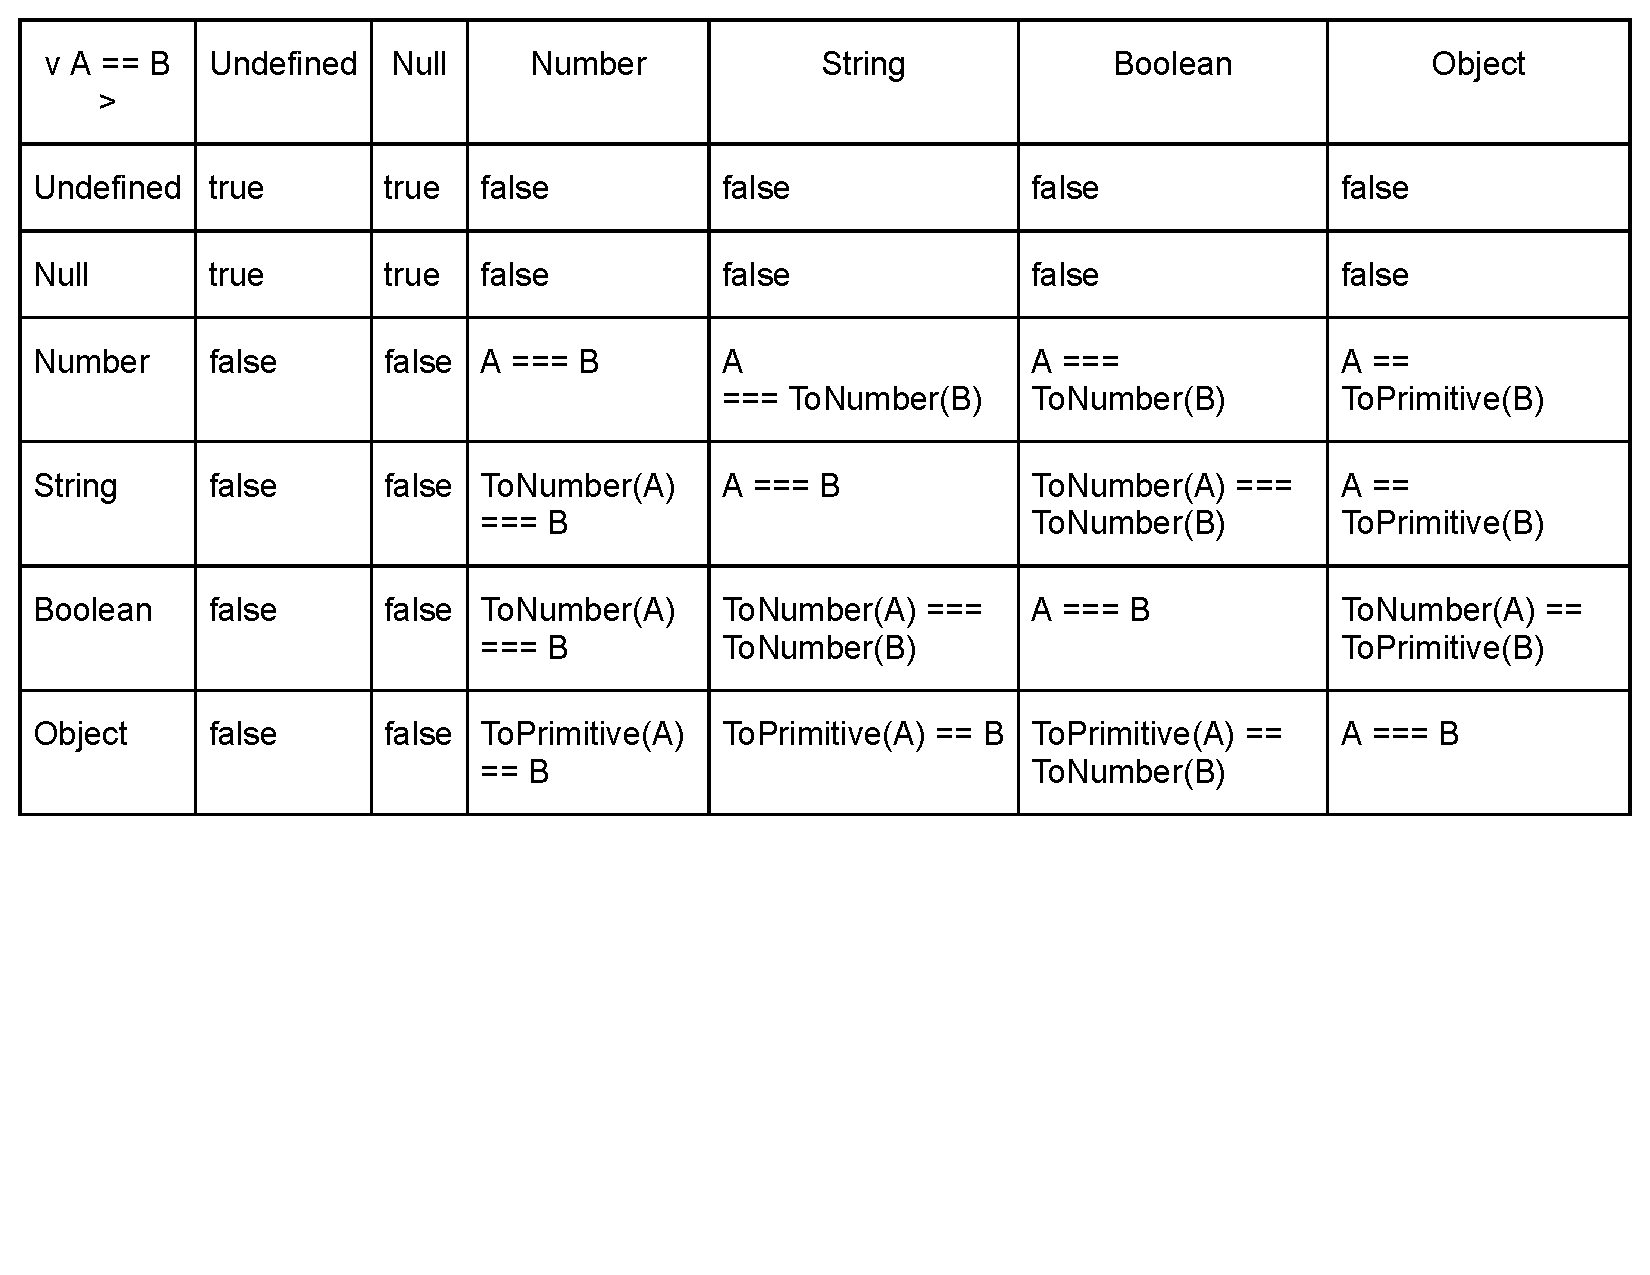
\includegraphics[scale = 0.2, trim={0 7.5cm, 0 0},clip]{equality.pdf}

Achtung: \mintinline{js}{0 == null}

\subsection{Array}

\begin{minted}{js}
var arr = [ 'a', 'b', 'c' ];
arr.forEach(function(elem, index){
  console.log(index +":"+elem);
});
\end{minted}

\subsection{Object}

Ein Object ist eine Sammlung von Properties. Die Properties werden mit einem Set (HashSet) verwaltet. Objekt können als ''object literals'' erstellt werden und/oder nachträglich mit Properties ergänzt werden.

\begin{minted}{js}
const person = {
  name : 'Markus',
  hallo : function(){ return 'Hallo '+this.name; }
};

console.log(person.name); // Markus
console.log(person['name']); // Markus
for (var property in dataObject) {} // foreach Attribute
\end{minted}

Falls eine Funktion als Methode von einem Objekt aufgerufen wird, ist this = Objekt. Beispiel: \mintinline{js}{object.foo();} Falls eine Funktion mit \mintinline{js}{new()} aufgerufen wird, wird «this» mit einem neu erstellten Objekt abgefüllt. Beispiel: \mintinline{js}{new foo();}. Spezialfall: \mintinline{js}{func.apply(obj)} ist gleichbedeutend mit \mintinline{js}{obj.func()}.

\subsection{Funktionen}

\begin{minted}{js}
function helloWorld3(...args) {
  console.log('helloWorld3', args);
}
function calc(fn, a, b=5){
  console.log(fn(a,b));
}
const filteredArray = array.filter( elem => elem > 5);
\end{minted}
Funktionsdefinitionen sollten in const Variablen abgespeichert werden, da sie sich ansonsten überschreiben lassen. fn.name beinhaltet den Namen und fn.length beinhaltet die Anzahl Parameter und fn.toString() gibt den Source Code der Funktion zurück.

\subsubsection{Scope}

Jede Funktion generiert einen neuen Scope. Innerhalb eines Scopes kann man auf dessen Variablen, globale Variablen und Variablen aller Parent-Scopes zugreifen. Variablendeklarationen werden immer an den Anfang des Blocks gelegt (\textbf{hoisting}).

Variablen ohne Keyword: nicht verwenden, bubblen nach oben. \mintinline{js}{var} bubblet hoch bis zur ersten Funktion, \mintinline{js}{let bzw. const} bleiben innerhalb des Blocks. Achtung: im globalen Scope hängen sich \mintinline{js}{var}-Variablen an \mintinline{js}{window.}, \mintinline{js}{let\/const} nicht.

\subsubsection{IIFE (Immediately Invoked Functional Expressions)}

\begin{minted}{js}
(function () {
  var localVar = 'action';
  console.log('IIFE in ' + localVar );
}());
\end{minted}

\subsection{Event Handler}
\begin{minted}{js}
<button onclick="bla()"></button>
button.onclick = fVar;
button.addEventListener("click", fVar);
// v with event capturing
button.addEventListener("click", fVar, true);
$('#id').click(fVar); // jQuery
container.on("click", "button", () => {})
// ^ falls .title-header dynamisch (z.B. Handlebars)
\end{minted}

Event Bubbling geht von innen nach aussen (Standard), Event Capturing von aussen nach innen.

Event-Listener sind nicht mehr aktiv wenn ein Element aus dem DOM-Tree entfernt wird. Es können aber Memory-Leaks entstehen bei dieser Art der "harten" Deregistierung. Besser: \mintinline{js}{.removeEventListener("event", Funktionsreferenz)}

\subsection{Handlebars}
\begin{minted}{html}
<script id="templ" type="text/x-handlebars-template">
  {{#each this}}
    <li> {{ firstName }} {{ lastName }} </li>
  {{/each}}
</script>
\end{minted}
\begin{minted}{js}
const customers = [
  {firstName:”Peter”, lastName:”Pan”, age:13},
  {firstName:”Captain”, lastName:”Hook”, age:35}
];
const createHTML = 
  Handlebars.compile($('#templ').html());
$('#container').html(createHTML(customers));
Handlebars.registerHelper('dateFormat', 
  (date, format) => { return moment(date, format) }
// {{ dateFormat someDate 'YYYY' }}
\end{minted}

\subsection{Promise}
\begin{minted}{js}
function sleep (time) {
  return new Promise((callback) => 
    setTimeout(callback, time));
}
sleep(1000).then(decrementCountDown);
\end{minted}

\subsection{AJAX}
scheme://authority/path?query\#fragment

\begin{minted}{js}
var request = new XMLHttpRequest();
request.onreadystatechange = () => {
var status = request.status;
if (request.readyState == 4 && (status == 200 )) {
    linkElement.parentNode.innerHTML = 
      request.responseText;
  }
};
request.open("GET", url); request.send();
$.get("some/url/", (data, jqXHR) => 
  { /* data available */ });
$.get("some/url").then(data => {})
\end{minted}

\subsection{CSS-Selektoren}
Elemente finden, die den CSS-Selektoren entsprechen: \mintinline{js}{node.querySelector[All](<selector>)}. Die normale Variante liefert den \textbf{ersten} Match, die \mintinline{js}{All}-Variante liefert eine NodeList. Dazu gibt es noch \mintinline{js}{document.getElementById()} und \mintinline{js}{document.getElementsByClassName()}.

\section{Usability}

Gute Usability ist ein System mit den Eigenschaften Effektivität, Effizienz und Zufriedenheit.

\subsection{Prinzipen der Dialoggestaltung ISO 9241-110}

\textbf{Aufgabenangemessenheit} Benutzer erledigen Aufgaben effektiv und effizient. \textbf{Selbstbeschreibungsfähigkeit} Dialogschritte sind durch Beschreibungen oder Rückmeldungen verständlich erklärt. \textbf{Steuerbarkeit} Benutzer kann Richtung und Geschwindigkeit der Interaktion beeinflussen. \textbf{Erwartungskonformität} Dialog entspricht den Kenntnissen des Benutzers. \textbf{Fehlertoleranz} Trotz erkennbarer fehlerhafter Eingaben des Benutzers kann das Ziel effizient erreicht werden. \textbf{Individualisierbarkeit} Interaktion kann angepasst werden. \textbf{Lernförderlichkeit} Erlernen der Anwendung wird unterstützt.

\subsection{Stone} \textbf{Visibility} der erste Schritt zum Ziel ist sichtbar. \textbf{Affordance (Begreifbarkeit)} Aktionsresultat ist vorhersagbar. \textbf{Feedback} Es ist klar was passiert ist (oder passiert => Animation). \textbf{Simplicity} Nicht mehr als nötig für die Aufgabe. \textbf{Structure} Logische und konsistente Organisation. \textbf{Consistency} Vorhersagbarkeit durch Konsistenz. \textbf{Tolerance} Fehler vermeiden, Wiederherstellung vereinfachen. \textbf{Accessibility} Design für alle Personengruppen \& Situationen

\section{Garrett}
\textbf{Oberfläche (sensorisches Design)} Sehschwächen, ältere Menschen, Farben (nicht mehr als 4 Farben $2+1$), Typografie, Icons. \textbf{Raster (Informationsdesign)} Strukturierung von Text und Information, Change Blindness beachten, Eye Catcher verwenden. Interaktionselemente müssen sichtbar sein (Long Press/Rechtsklick kritisch). \textbf{Struktur (Interaktion)} Informationsarchitektur. Die Nutzer müssen stets wissen: wo bin ich im Moment, wo kann ich hin, was ist passiert. Vorgehen: \textbf{Card Sorting} (Herangehensweise zur Kategorisierung)

\section{User Centered Design:}
Untere beide Garrett-Ebenen, \textbf{Umfang (Inhaltsanforderung)} mit Anforderungsanalyse. \textbf{Strategie (Nutzerbedürfnisse)} mit Marktanalyse, Zielgruppenanalyse

Benutzerbefragung ist kein User Centered-Design, Nutzer wissen eigentlich nicht was sie wollen. 

Wichtige Axiome: Benutzer sind Experten in ihrem Kontext und in ihrer Welt. Designer und Techniker sind Experten darin, wie die Welt sein könnte. Vor dem besser machen, muss die alte Welt verstanden werden.

\textbf{Analyse} Benutzer und Kontext verstehen

\textbf{Modellieren} Entwurf und Optimierung einer passenden Lösung

\textbf{Spezifikation} die Lösung in die Entwicklung tragen

\textbf{Realisierung} (Unterstützung bei der) Implementierung der Lösung

\textbf{Evaluation} Resultate mit Benutzern überprüfen

\end{multicols*}
\end{document}
